\subsection{Langkah Praktikum: Branch and Bound pada TSP}
Praktikum 8 menerapkan Branch and Bound untuk TSP. Graf berbobot diubah menjadi matriks biaya, lalu cabang dengan bound terkecil diproses lebih dahulu.

\begin{figure}[H]
    \centering
    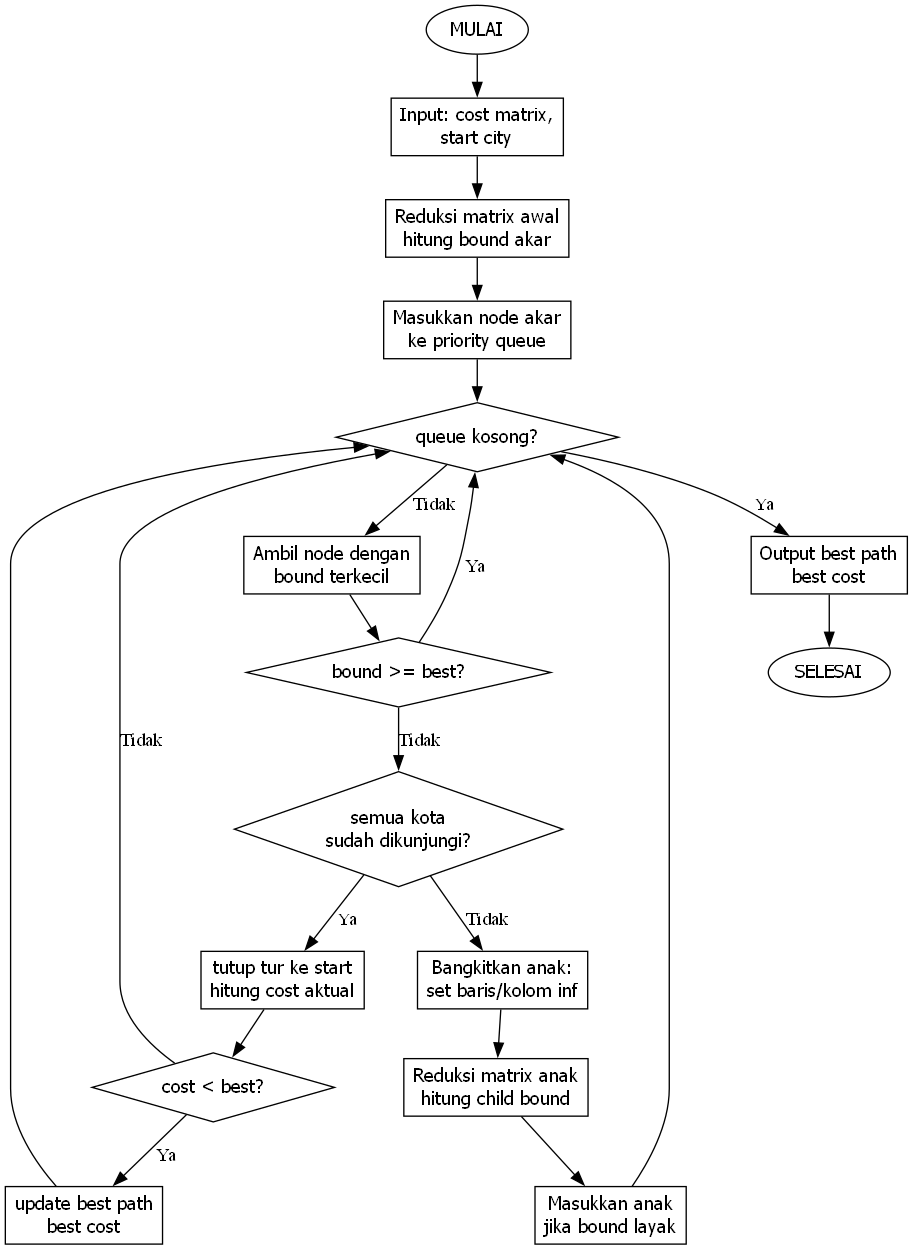
\includegraphics[width=0.55\textwidth]{figures/praktikum8/flowchart_branch_bound_tsp.png}
    \caption{Flowchart Branch and Bound untuk TSP}
    \label{fig:praktikum8-flowchart-bnb}
\end{figure}

\subsubsection*{Source Code Python}
Source code lengkap terdapat pada folder \texttt{src/praktikum8}. Bagian berikut hanya menampilkan inti program.

\textbf{1. Fungsi reduksi cost matrix}
\begin{lstlisting}[basicstyle=\ttfamily\scriptsize, frame=single, backgroundcolor=\color{white}, numbers=none, keywordstyle=\color{black}, commentstyle=\color{black}, stringstyle=\color{black}, breaklines=true]
def reduce_matrix(matrix):
    reduction_cost = 0
    num_nodes = len(matrix)

    for row in matrix:
        finite_values = [value for value in row if value != inf]
        if not finite_values:
            continue
        minimum = min(finite_values)
        if minimum > 0:
            reduction_cost += minimum
            for col_idx in range(num_nodes):
                if row[col_idx] != inf:
                    row[col_idx] -= minimum

    for col_idx in range(num_nodes):
        finite_values = [
            matrix[row_idx][col_idx]
            for row_idx in range(num_nodes)
            if matrix[row_idx][col_idx] != inf
        ]
        if not finite_values:
            continue
        minimum = min(finite_values)
        if minimum > 0:
            reduction_cost += minimum
            for row_idx in range(num_nodes):
                if matrix[row_idx][col_idx] != inf:
                    matrix[row_idx][col_idx] -= minimum

    return reduction_cost
\end{lstlisting}

\textbf{2. Fungsi utama Branch and Bound TSP}
\begin{lstlisting}[basicstyle=\ttfamily\scriptsize, frame=single, backgroundcolor=\color{white}, numbers=none, keywordstyle=\color{black}, commentstyle=\color{black}, stringstyle=\color{black}, breaklines=true]
def branch_and_bound_tsp(cost_matrix, start_city=0):
    root_matrix = copy_matrix(cost_matrix)
    root_bound = reduce_matrix(root_matrix)
    queue = [SearchNode(root_bound, 0, start_city, [start_city], root_matrix)]

    best_cost = inf
    best_path = []

    while queue:
        node = heappop(queue)
        if node.bound >= best_cost:
            continue

        if node.level == len(cost_matrix) - 1:
            candidate_path = node.path + [start_city]
            candidate_cost = path_cost(cost_matrix, candidate_path)
            if candidate_cost < best_cost:
                best_cost = candidate_cost
                best_path = candidate_path
            continue

        for next_city in range(len(cost_matrix)):
            if next_city in node.path:
                continue

            child_matrix = copy_matrix(node.matrix)
            edge_cost = child_matrix[node.current_city][next_city]
            if edge_cost == inf:
                continue

            for city in range(len(cost_matrix)):
                child_matrix[node.current_city][city] = inf
                child_matrix[city][next_city] = inf
            child_matrix[next_city][start_city] = inf

            child_bound = node.bound + edge_cost + reduce_matrix(child_matrix)
            if child_bound < best_cost:
                heappush(queue, SearchNode(
                    child_bound, node.level + 1, next_city,
                    node.path + [next_city], child_matrix
                ))

    return best_path, best_cost
\end{lstlisting}

\textbf{3. Kode tester}
\begin{lstlisting}[basicstyle=\ttfamily\scriptsize, frame=single, backgroundcolor=\color{white}, numbers=none, keywordstyle=\color{black}, commentstyle=\color{black}, stringstyle=\color{black}, breaklines=true]
praktikum_edges = [
    (0, 1, 12), (0, 2, 10), (0, 3, 5),
    (1, 2, 9), (1, 3, 8), (2, 3, 15),
]

pretest_edges = [
    (0, 1, 25), (0, 2, 15), (0, 3, 20),
    (1, 2, 35), (1, 3, 10), (2, 3, 30),
]

run_case("Graf praktikum Gambar 8.1", 4, praktikum_edges)
run_case("Graf pre/post test Gambar 8.3", 4, pretest_edges)
\end{lstlisting}

\subsubsection*{Analisis}
\textbf{Hasil graf praktikum:}
\begin{table}[H]
    \centering
    \caption{Hasil Branch and Bound pada Graf Contoh Praktikum}
    \label{tab:praktikum8-hasil-praktikum}
    \begin{tabular}{ll}
    \toprule
    \textbf{Aspek} & \textbf{Hasil} \\ \midrule
    Jumlah simpul & 4 \\
    Start & 0 \\
    Jalur minimum & [0, 2, 1, 3, 0] \\
    Cost minimum & 32 \\
    Simpul diekspansi & 6 \\
    Simpul dipangkas & 4 \\ \bottomrule
    \end{tabular}
\end{table}

\textbf{Post Test: TSP pada Graf Gambar 8.3}
\begin{table}[H]
    \centering
    \caption{Validasi Hasil Program vs Manual pada Graf Gambar 8.3}
    \label{tab:praktikum8-validasi-posttest}
    \begin{tabular}{lll}
    \toprule
    \textbf{Sumber} & \textbf{Jalur Minimum} & \textbf{Cost Minimum} \\ \midrule
    Manual Pre Test & 0--2--1--3--0 & 80 \\
    Program Python & [0, 2, 1, 3, 0] & 80 \\ \bottomrule
    \end{tabular}
\end{table}

\textbf{Kesimpulan:} Program menghasilkan cost minimum yang sama dengan perhitungan manual. Pada graf Gambar 8.3 terdapat beberapa rute dengan cost 80, sehingga salah satu rute minimum sudah cukup valid.
